\documentclass[default,compress]{beamer}

%\usepackage[utf8]{inputenc}
\usepackage{beamerthemesplit}
%\usepackage{textcomp}
%\usepackage{epsfig}
\usepackage{amsmath}
\usepackage{amssymb}
\usepackage{graphicx}
\usepackage{textpos}

\usepackage{units}


%\usepackage{multimedia}
%\usepackage{tikz}
%\usepackage{pdflscape}
\usepackage{multicol}
\usepackage{minted}


\hypersetup{
    colorlinks=true, % false: boxed links; true: colored links
    urlcolor=black    % color of external links
}

\mode<presentation>

\setbeamertemplate{navigation symbols}{}

%\title{Building an open source Python ecosystem for plasma physics}
\title{The PlasmaPy Project:\ Building an open source software ecosystem for plasma science}
\author{Nick Murphy\inst{1} on behalf of the PlasmaPy Community}
\institute{\inst{1}Center for Astrophysics $\vert$\ Harvard \& Smithsonian}
\date{\small{
1st Computational Physics School for Fusion Research\\
August 28, 2019}}

\begin{document}

%%%%%%%%%%%%%%%%%%%%%%%%%%%%%%%%%%%%%%%%%%%%%%%%%%%%%%%%%%%%%%%%%%%%%%%%

\begin{frame}[plain]

    \titlepage

    \begin{textblock}{1}(-0.9,0.5)
      \href{http://www.plasmapy.org/}{
\includegraphics[height=0.57cm]{plasmapy-logo.png}}
    \end{textblock}
    
    \begin{textblock}{1}(12.4,0.5)
      \href{https://creativecommons.org/licenses/by/4.0/}{
\includegraphics[height=0.57cm]{by.png}}
    \end{textblock}
    
\end{frame}


\begin{frame}[plain]
    \frametitle{Plasma physics has a ``roll your own'' culture for software development}
    \begin{itemize}
    \item Software usually developed ``in-house'' as needeed
    \item Duplication, triplication, \& quadruplication of functionality
    \item We tend to be self-taught as programmers
    \item Time pressure prevents us from learning how to improve programming skills
    \item Code is often written in a rush to get a paper out
    \item Code is often written for a specific purpose, which makes it hard to generalize
    \item Documentation is often insufficient
    \item Codes often lack a testing framework
    \item Packages lack interoperability
    \item Access to codes is often restricted in some way
    \end{itemize}
\end{frame}


\begin{frame}[plain]
    \frametitle{Consequences of ``roll your own'' culture}
    \begin{itemize}
    \item \textbf{Beginning research is difficult} due to software overhead
    \item \textbf{Collaboration is difficult} due to lack of interoperability
    \item Plasma research is much \textbf{less reproducible}
    \item Research can be \textbf{frustrating}
    \end{itemize}
        \vspace{3mm}
    \begin{center}
        \fbox{\parbox{100mm}{\Large{
            We can learn from what other fields are doing to change ``roll your own'' culture.
            }
        }}
    \end{center}

\end{frame}


\begin{frame}[plain]

    \frametitle{Astronomy's response to ``roll your own'' culture is Astropy}
    \begin{center}
        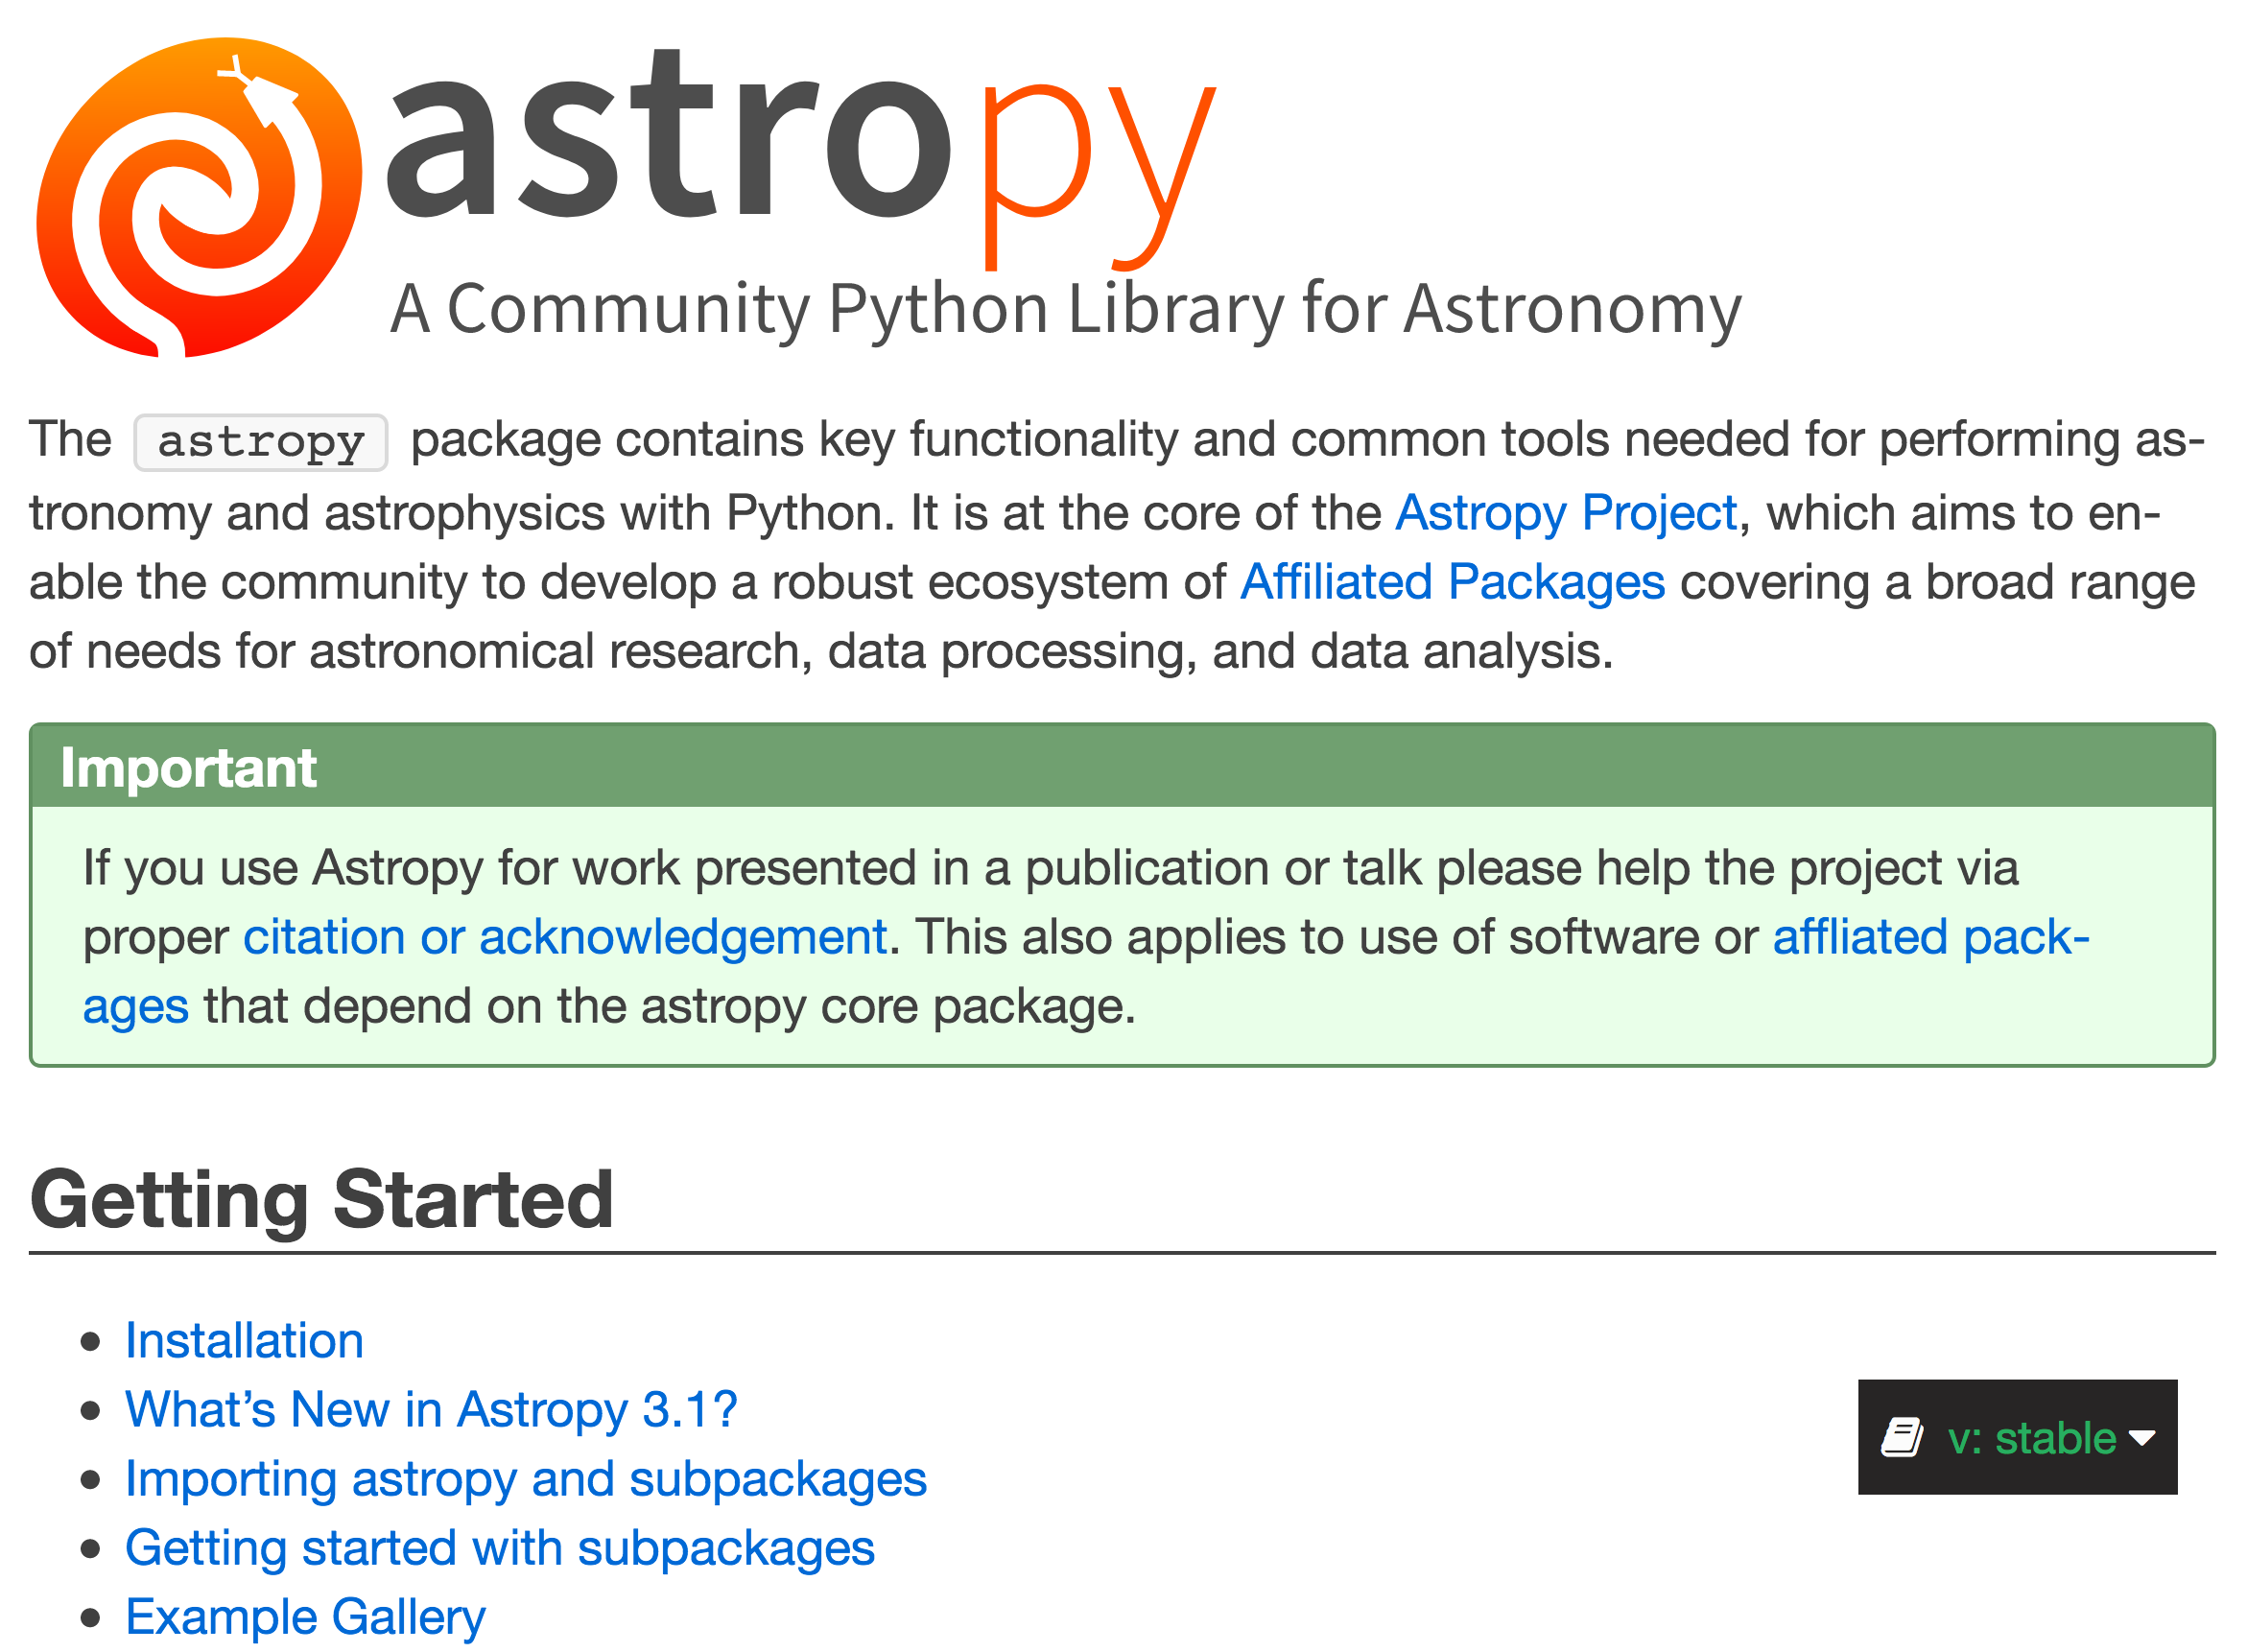
\includegraphics[width=11.0cm]{AstropyDocsHeader.png}
    \end{center}

\end{frame}


\begin{frame}[plain]
    \frametitle{Astropy is a software package and a project}
    \begin{itemize}
    \item The \textbf{Astropy package} contains functionality needed by most astronomers
        \begin{itemize}
        \item Units, coordinates, etc.
        \end{itemize}
    \item Astropy \textbf{affiliated packages} contain specialized functionality
        \begin{itemize}
        \item Spectroscopy, galactic dynamics, etc.
        \end{itemize}
    \item The \textbf{Astropy Project} coordinates the core and affiliated packages
    \end{itemize}
    \vspace{2mm}
    \begin{center}
        \fbox{\parbox{100mm}{\large{
            \begin{center}
                Astropy and affiliated packages constitute an openly developed \textbf{software ecosystem} for astronomy
            \end{center}
            }}}
    \end{center}
\end{frame}


\begin{frame}[plain]
    \frametitle{The goal of the PlasmaPy project is to facilitate an open source software ecosystem for plasma research \& education}
    \begin{center}
        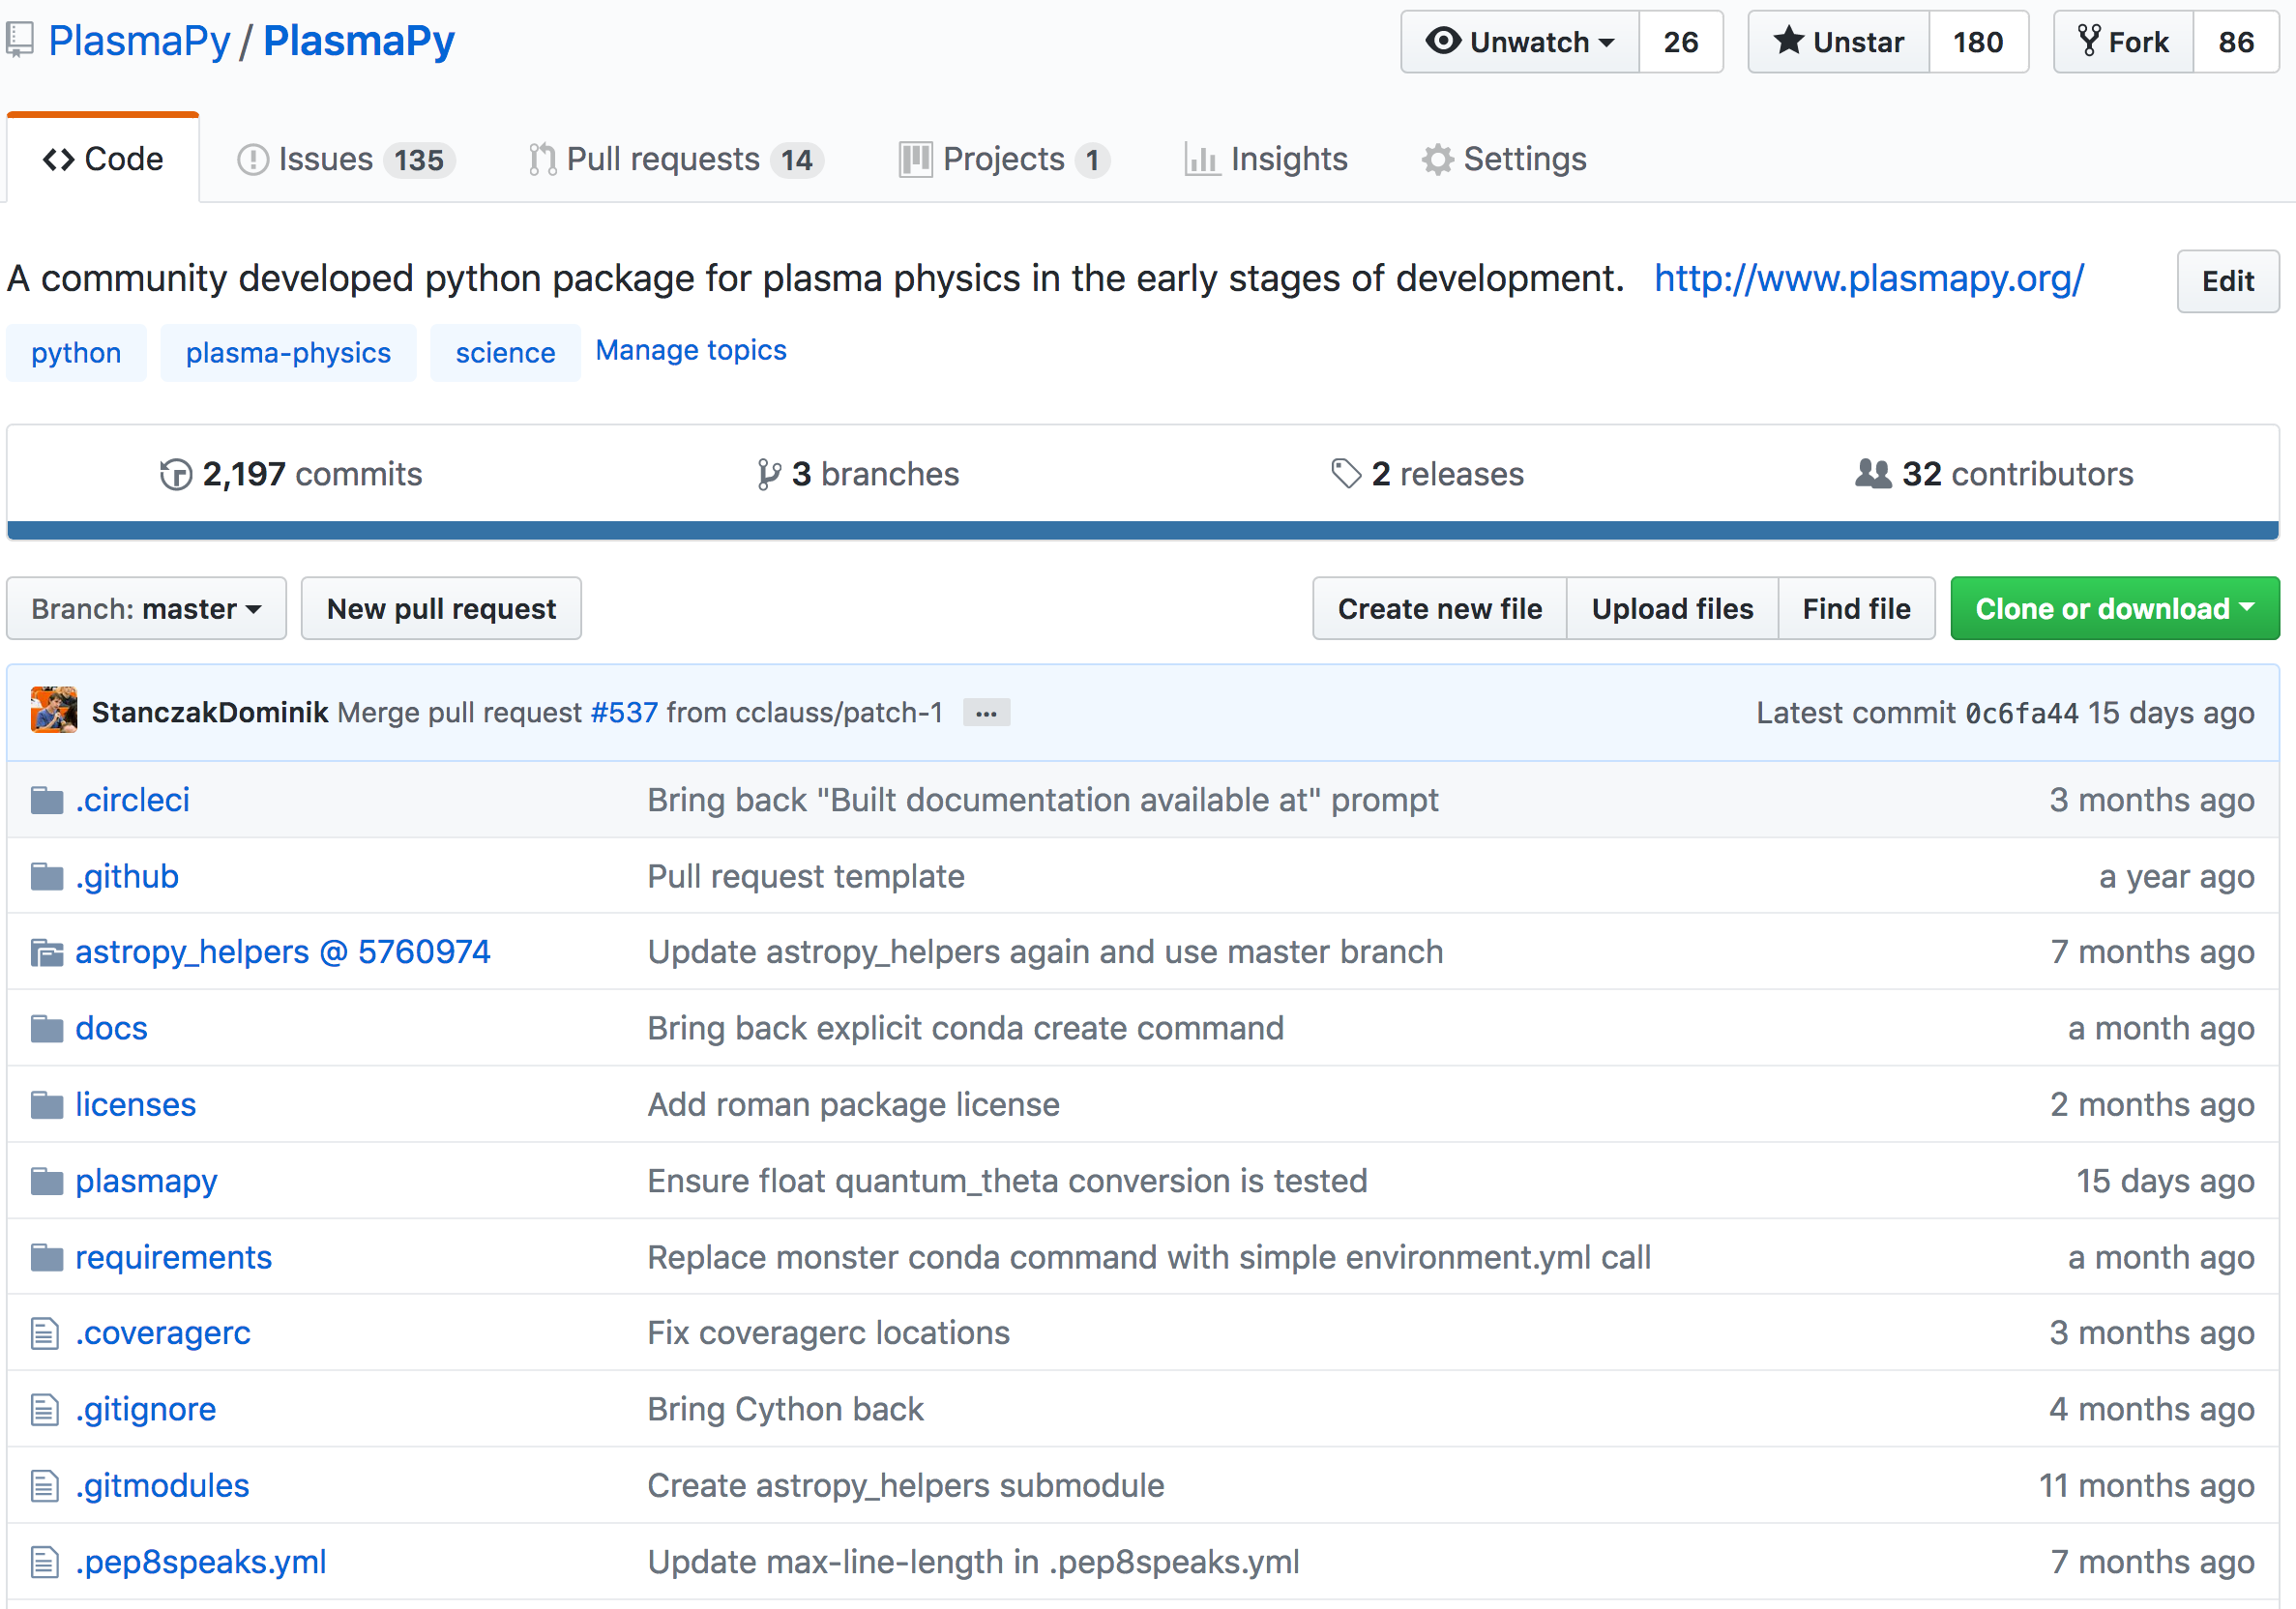
\includegraphics[width=11.0cm]{PlasmaPy_mainpage.png}
    \end{center}
\end{frame}


\begin{frame}[plain]
    \frametitle{PlasmaPy is open source for open and reproducible science}
    \begin{itemize}
    \item PlasmaPy is released under the Open Source Initiative approved \textbf{BSD+Patent license}
        \begin{itemize}
        \item Can freely use, modify, and redistribute code as long as you include a copy of the license
        \item Provides protections for users against software patents
        \end{itemize}
    \end{itemize}
\end{frame}


\begin{frame}[plain]
    \frametitle{Early development of PlasmaPy through version 0.2.0}
    \begin{itemize}
    \item Wrote a vision statement
    \item Adopted a code of conduct
    \item Developed organizational infrastructure 
    \item Created package infrastructure
    \item Set up documentation \& testing frameworks
    \item Set up interfaces to access basic atomic data
    \item Implemented much of the \emph{NRL Plasma Formulary}
    \item Began prototyping diagnostic analysis classes
    \item Created machinery for base class factory\footnote{Thanks to Google Summer of Code 2018 student Ritiek Malhotra!}
    \end{itemize}
\end{frame}


\begin{frame}[plain]
    \frametitle{PlasmaPy subpackages in version 0.2.0}
    \begin{itemize}
    \item \mintinline{python}{atomic} allows access to basic atomic data
    \item \mintinline{python}{classes} contains prototype base classes
    \item \mintinline{python}{constants} provides physical constants
    \item \mintinline{python}{diagnostics} will provide experimental analysis tools
    \item \mintinline{python}{mathematics} contains oft-needed analytical functions
    \item \mintinline{python}{physics} calculates plasma parameters
    \item \mintinline{python}{transport} calculates classical transport coefficients
    \item \mintinline{python}{utils} provides utilities used throughout the package
    \end{itemize}
\end{frame}


\defverbatim[colored]\AstropyUnits{\vspace{-2mm}
    \begin{minted}[fontsize=\normalsize,
                   framesep=3mm,
                   autogobble,
                   ]{pycon}
    >>> from astropy import units
    
    >>> distance = 44 * units.imperial.mile
    >>> time = 30 * units.minute
    >>> distance / time
    <Quantity 88.0 mi / h>

    >>> (1.21 * units.GW).cgs
    <Quantity 1.21e+16 erg / s>
    
    >>> 2 * units.m + 4 * units.m / units.s
    UnitConversionError: Can only apply 'add' function 
    to quantities with compatible dimensions
    \end{minted}
}

\begin{frame}[plain]
    \frametitle{PlasmaPy uses the \href{http://docs.astropy.org/en/stable/units/}{\mintinline[style=fruity]{python}{astropy.units}} package for units}
    This package creates \mintinline{python}{Quantity} objects with attached units.\\ 
    \AstropyUnits
\end{frame}


\defverbatim[colored]\AstropyUnitsCooking{
    \begin{minted}[fontsize=\large,
                   framesep=3mm,
                   autogobble
                   ]{pycon}
    >>> volume = 1 * units.barn * units.Mpc
    >>> volume.to(units.imperial.tsp)
    <Quantity 0.62603503 tsp>
    \end{minted}
}

\begin{frame}[plain]
    \frametitle{\texttt{astropy.units} is great if you want to write a cookbook with ridiculous units}
    \AstropyUnitsCooking
\end{frame}


\defverbatim[colored]\atomic{
    \begin{minted}[fontsize=\normalsize,
                   framesep=3mm,
                   style=emacs,
                   autogobble
                   ]{pycon}
    >>> from plasmapy.atomic import Particle
    
    >>> alpha = Particle("He-4++")
    >>> alpha.mass
    <Quantity 6.64465709e-27 kg>
    
    >>> electron = Particle("e-")
    >>> electron.charge
    <Quantity -1.60217662e-19 C>
    >>> electron.is_category(require={"lepton", "fermion"})
    True
    >>> ~electron  # find antiparticle with invert operator
    Particle("e+")
    \end{minted}
}

\begin{frame}[plain]
    \frametitle{PlasmaPy's \mintinline{python}{atomic} subpackage provides functional and object-oriented interfaces to particle data}
    Instances of the \mintinline{python}{Particle} class may be used to represent individual atoms, ions, or elementary particles.
    \\ \vspace{-2mm}
    \atomic
\end{frame}


\defverbatim[colored]\physics{
    \begin{minted}[fontsize=\normalsize,
                   framesep=3mm,
                   style=emacs,
                   autogobble
                   ]{pycon}
    >>> from plasmapy.physics import *
    
    >>> n_e = 1e15 * units.m ** -3
    >>> T_e = 6 * units.MK
    >>> B = 0.2 * units.T
    
    >>> Debye_length(n_e, T_e)
    <Quantity 0.00534541 m>
    
    >>> upper_hybrid_frequency(B, n_e)
    <Quantity 3.52216092e+10 rad / s>
    
    >>> n_i = 5e19 * units.m ** -3
    >>> inertial_length(n_i, 'D+')
    <Quantity 0.04553085 m>  
    \end{minted}
}

\begin{frame}[plain]
    \frametitle{The \mintinline{python}{physics} subpackage provides functions to calculate plasma parameters}
    \physics
\end{frame}



\defverbatim[colored]\classicaltransport{
    \begin{minted}[fontsize=\small,
                   framesep=3mm,
                   style=emacs,
                   autogobble
                   ]{pycon}
    >>> from plasmapy.transport import *
    >>> T = 1 * units.MK
    >>> n = 5e15 * units.m ** -3
    >>> particles = ('e-', 'p+')
    >>> collision_frequency(T, n, particles)
    <Quantity 443.02775451 Hz>
    >>> coupling_parameter(T, n, particles)
    <Quantity 4.60608476e-06>

    >>> T_e, n_e = 0.6 * units.keV, 1e16 * units.cm ** -3
    >>> T_p, n_p = 0.8 * units.keV, 1e16 * units.cm ** -3
    >>> braginskii = ClassicalTransport(T_e, n_e, T_p, n_p, 'p+')
    >>> braginskii.ion_thermal_conductivity
    <Quantity 132961.01785222 W / (K m)>
    >>> braginskii.electron_viscosity
    <Quantity [0.02734206, 0.02733305, 0.02733305, 0., 0.] Pa s>

    \end{minted}
}

\begin{frame}[plain]
    \frametitle{The \mintinline{python}{transport} subpackage provides functions to calculate collision parameters and transport coefficients}
    \classicaltransport
\end{frame}


\begin{frame}[plain]
    \frametitle{PlasmaPy has documentation!}
    \vspace{-1mm}
    \begin{center}
        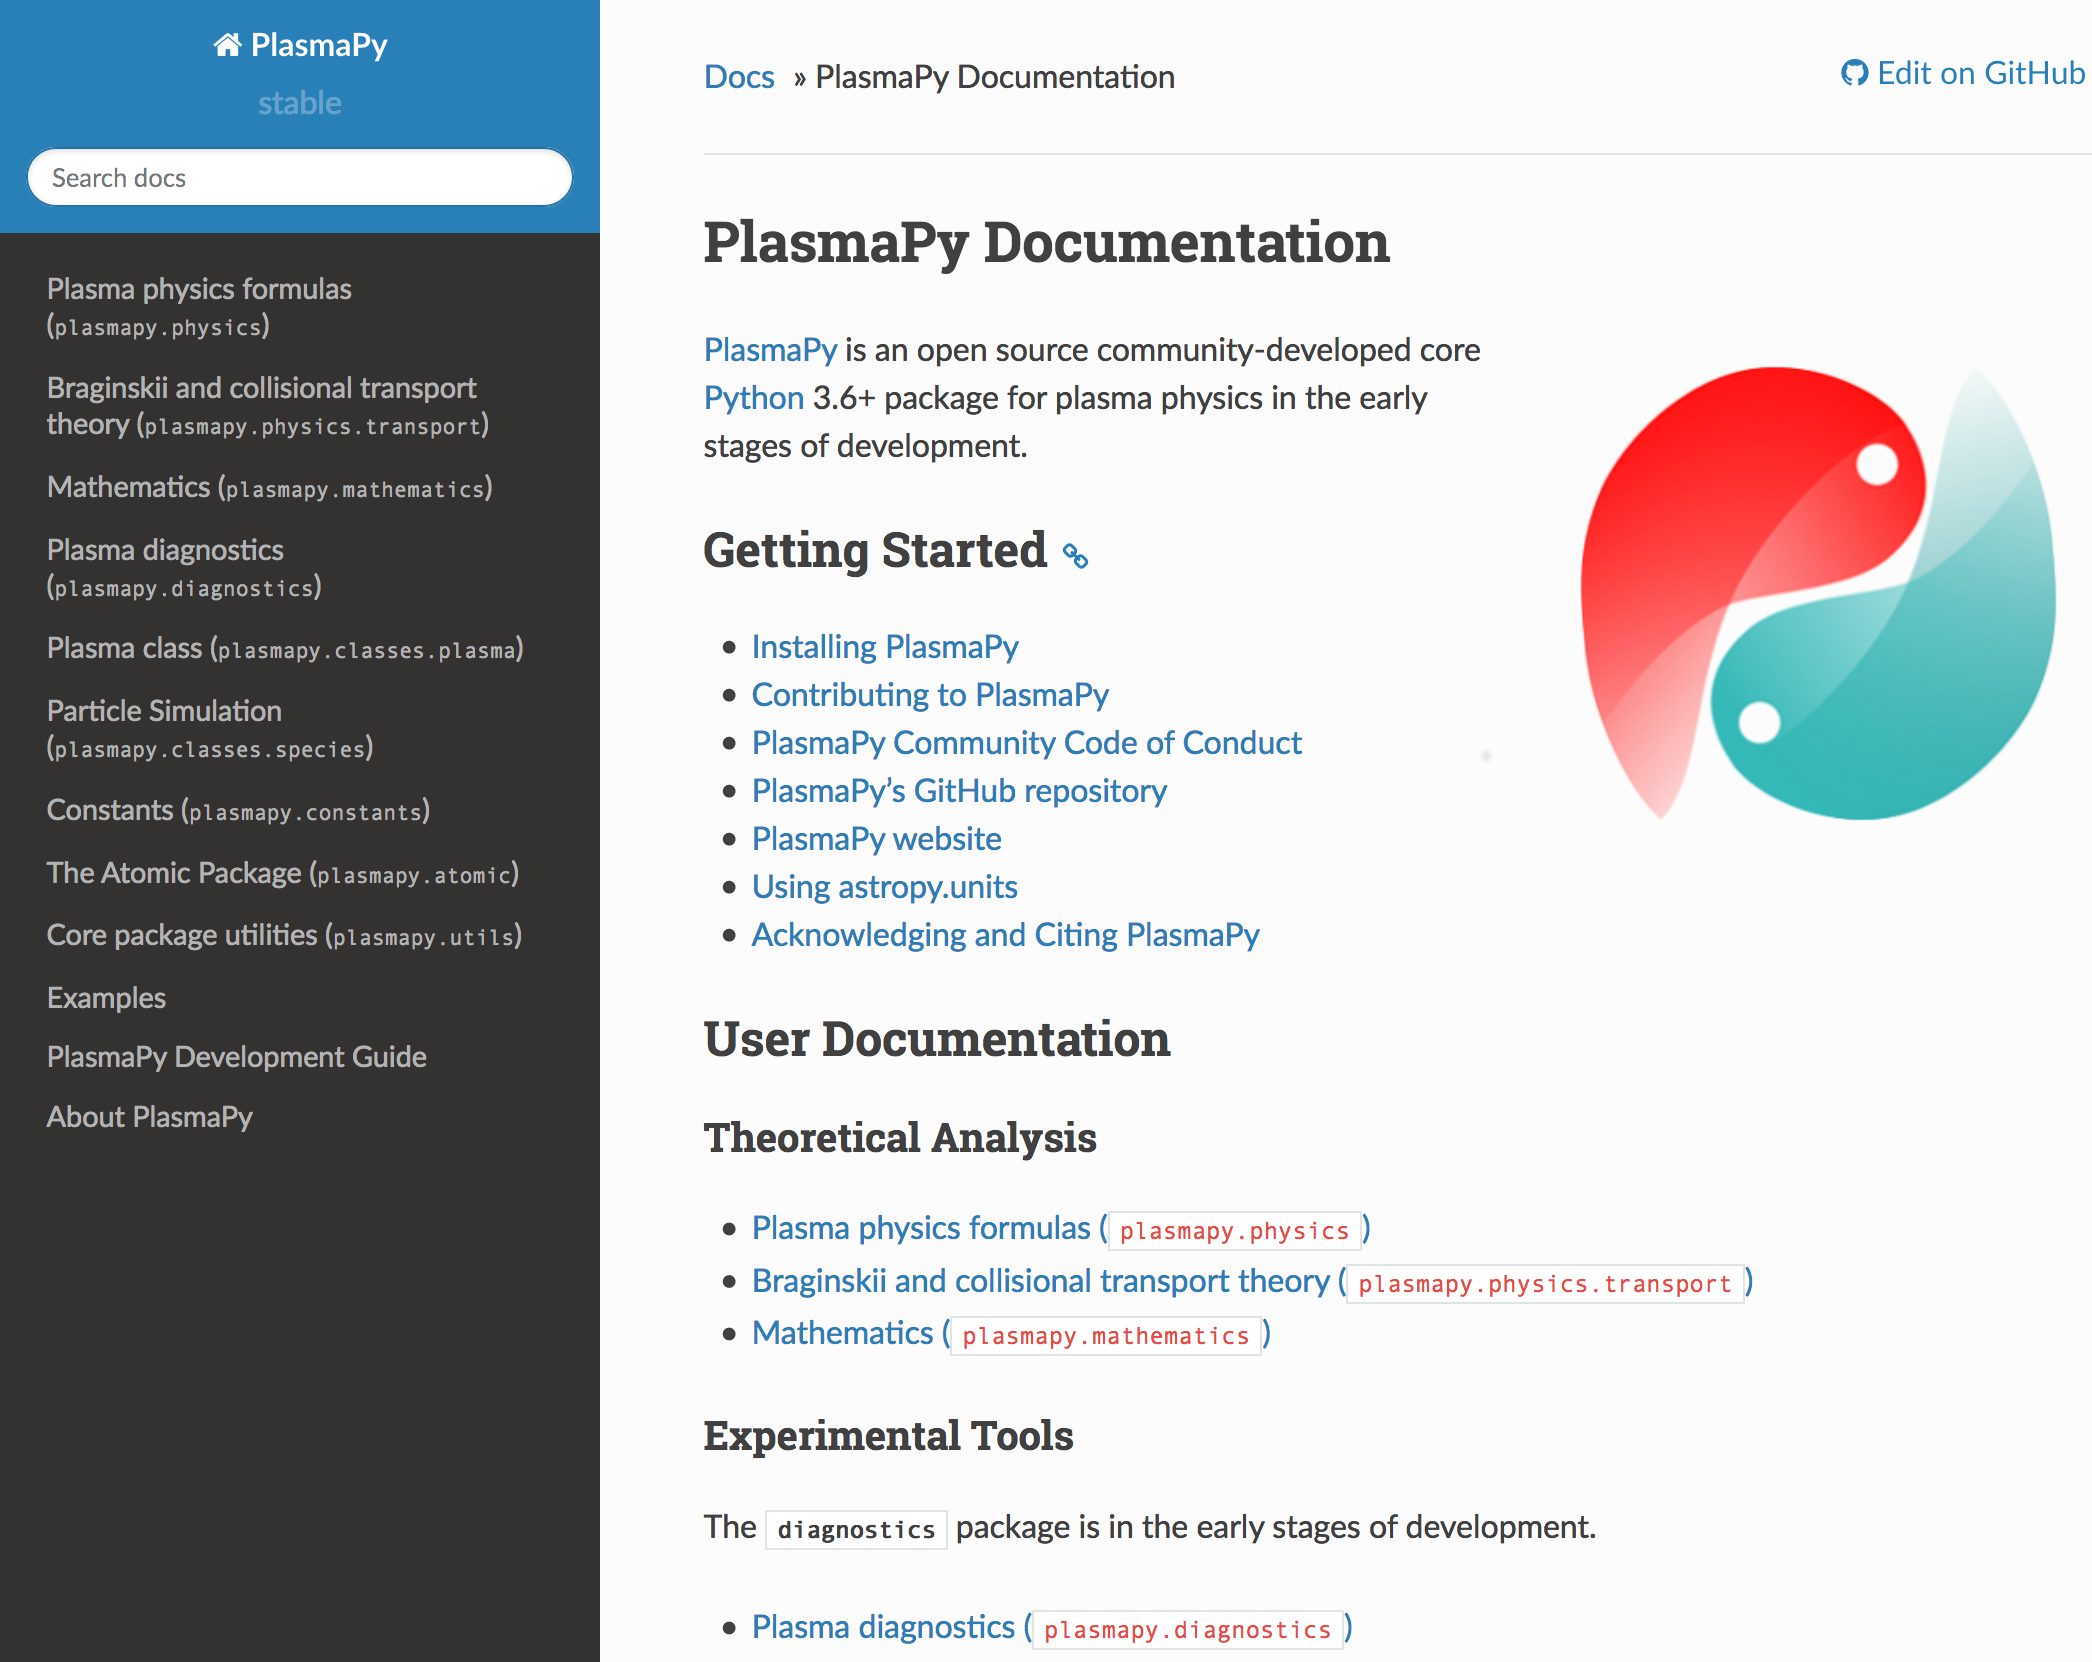
\includegraphics[height=8.7cm]{PlasmaPy_docs.png}
    \end{center}
\end{frame}


\begin{frame}[plain]
    \frametitle{PlasmaPy has tests!}
    \begin{center}
        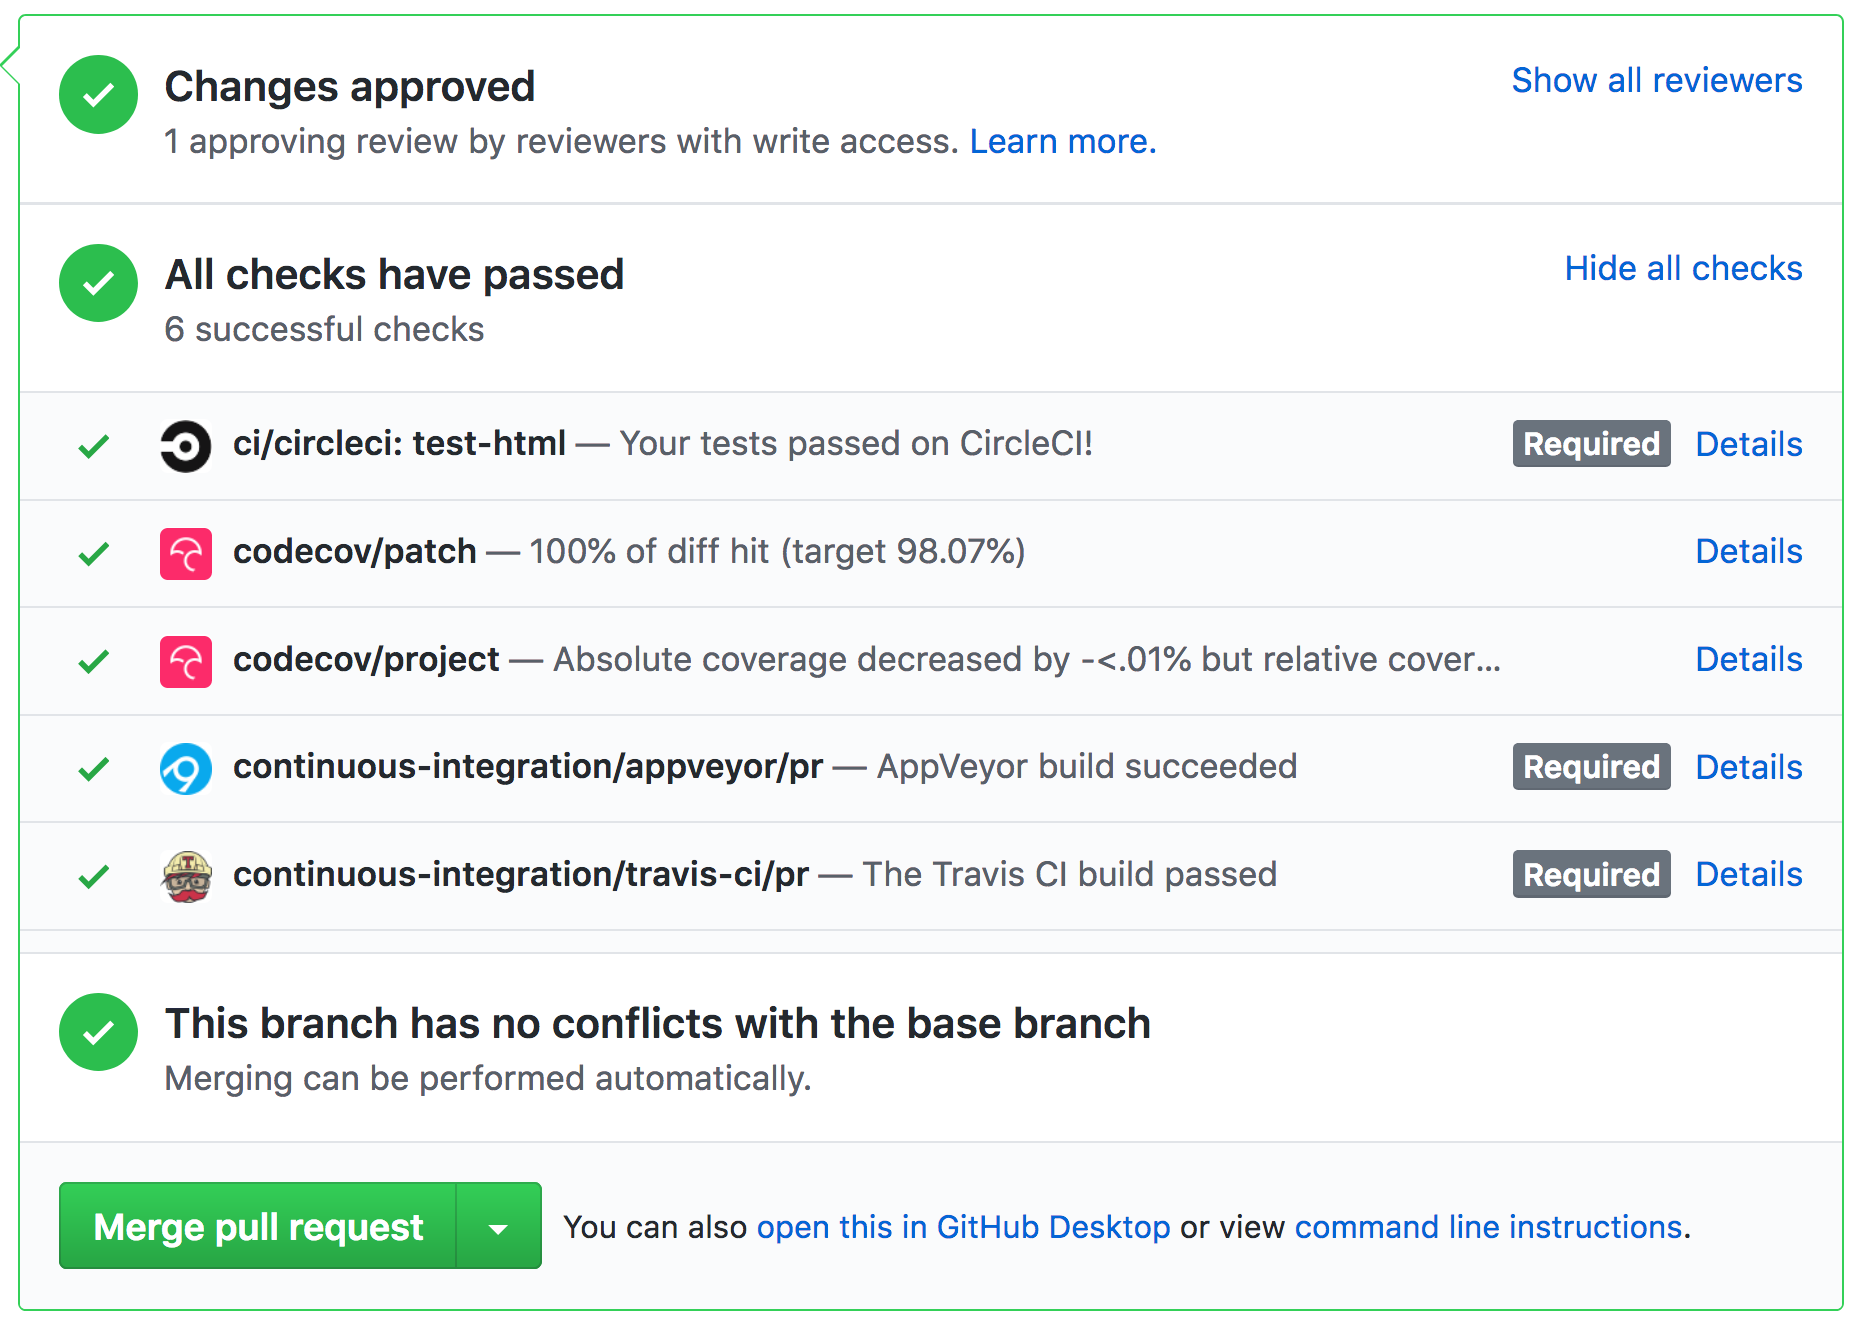
\includegraphics[height=7.8cm]{PlasmaPy_testsuite.png}
    \end{center}
\end{frame}


\begin{frame}[plain]
    \frametitle{Why do we need tests?}
    \begin{itemize}
    \item Benefits of a testing framework
        \begin{itemize}
        \item Improved confidence in software reliability
        \item Quicker to track down and fix bugs
        \item We can change our code quickly and verifiably
        \end{itemize}
    \item Consequences of not having a testing framework
        \begin{itemize}
        \item Decreased reliability
        \item Hidden bugs
        \item Reluctance to make changes for fear of breaking something
        \end{itemize}
%    \item Legacy code can be defined as \emph{code without tests}\footnote{From \emph{Working Effectively With Legacy Code} by Michael Feathers}
%    \item \textbf{Tests make code more flexible}
    \end{itemize}
\end{frame}


\begin{frame}[plain]
    \frametitle{Next steps as described in our NSF proposal\footnote{Murphy, Everson,  Vincena, Parashar, \& Schaffner (2019), \emph{An open source software ecosystem for plasma physics}, Zenodo, doi:10.5281/zenodo.3244419}}
    \begin{itemize}
    \item Create tutorials on how to use \& contribute to PlasmaPy
    \item Refactor existing code to improve long-term maintainability
    \item Improve testing framework
    \item Formalize software architecture
    \item Implement high level data structures
    \item Write a dispersion relation solver
    \item Develop experimental data analysis tools
    \item Create time series turbulence analysis tools
    \item Create foundation of plasma simulation framework (in Julia!)
    \end{itemize}
\end{frame}


\begin{frame}[plain]
    \frametitle{Challenges}
    \begin{itemize}
    \item Data access
        \begin{itemize}
        \item Most astronomical \& heliospheric data sets are open access
        \item Most laboratory plasma data sets are closed access
        \end{itemize}
%    \item Most astronomical data sets are open access
%    \item Access to most laboratory plasma data is restricted
%        \begin{itemize}
%        \item More difficult to create plasma analysis tools
%        \item Major barrier to data science studies
%        \end{itemize}
    \item We can make plasma science more open and reproducible
        \begin{itemize}
        \item Release experimental data sets under open access licenses
        \item Produce an online portal to access plasma data sets
        \item Collaborate on open metadata standards
        \end{itemize}
    \end{itemize}
\end{frame}

\begin{frame}[plain]
    \frametitle{Plasma physics is maybe not the most inclusive discipline}
    \begin{itemize}
    \item In the APS Division of Plasma Physics, $\sim$15\% of student members and $\sim$9\% of all members are women
        \begin{itemize}
        \item Limited data for additional dimensions of identity
        \end{itemize}
    \item This is a crisis, but is usually not treated as such
    \item Equity \& inclusion must be core to the PlasmaPy project
    \item Possibility:\ a conference on equity \& inclusion in plasma physics
        \begin{itemize}
        \item Must take an intersectional approach
        \end{itemize}
    \end{itemize}
\end{frame}

%\begin{frame}[plain]
%    \frametitle{Summary}
%    \begin{itemize}
%    \item We have begun developing PlasmaPy to become a core Python package for plasma physics
        %\begin{itemize}
        %\item We are using Astropy's model for open development
%        \item Please raise issues on GitHub for feature requests!
        %\end{itemize}
%    \item Open source software improves scientific reproducibility 
%    \item Best practices for scientific computing
%        \begin{itemize}
%        \item Write tests
%        \item Include documentation
%        \item Prioritize readability
%        \item Use version control
%        \item Collaborate
%        \item Build community
%        \end{itemize}
%%    \item We are still learning!
%    \end{itemize}
%\end{frame}\end{document}

\begin{frame}[plain]
    \frametitle{Final thoughts}
    \begin{itemize}
    \item Our community would benefit from an open source software ecosystem
        \begin{itemize}
        \item Improve interoperability
        \item Reduce quadruplication of functionality
        \item Promote community
        \item Make our lives easier
        \end{itemize}
    \item Julia and Python can co-exist
    \item Next generation plasma simulation software should be in Julia
        \begin{itemize}
        \item I have opinions!
        \end{itemize}
    \item We should take time to learn
        \begin{itemize}
        \item Software engineering best practices
        \item How to write clean code with clean architecture
        \end{itemize}
    \item \textbf{Code is communication!}
\end{itemize}
\end{frame}


\begin{frame}[plain]
    \frametitle{Becoming involved}
    \begin{itemize}

    \item Join conversation on Matrix channel
        \begin{center}
            {\color{blue}\small{
                \texttt{https://riot.im/app/\#/room/\#plasmapy:openastronomy.org}}}
        \end{center}
    \item Join PlasmaPy's email list
        \begin{center}
            {\color{blue}
            \small{\texttt{https://groups.google.com/forum/\#!forum/plasmapy}}
            }
        \end{center}
    \item Submit feature requests via GitHub issues, or contribute code, documentation, tutorials, and examples on our GitHub repository
        \begin{center}
            {\color{blue}
            \small{\texttt{https://github.com/PlasmaPy/plasmapy}}
            }
        \end{center}
    \item Organize community events
    \item Advocate for openness, reproducibility, equity, \& inclusion in plasma science
    \end{itemize}
\end{frame}

\begin{frame}[plain]
    \begin{center}
        
\includegraphics[height=4.9cm]{URSSI_winter_school.png}
        \\~\\
        \texttt{http://urssi.us/winterschool}
    \end{center}
\end{frame}

\end{document}
